\chapter{Solution of linear systems of equation}
\label{cha:solution_of_linear_systems}
\minitoc

This chapter is devoted to the numerical solution of linear problems of the following form:
\begin{equation}
    \label{eq:linear_system}
    \text{Find $\vect x \in \real^n$ such that} \qquad
    \mat A \vect x = \vect b,
    \qquad \mat A \in \real^{n \times n},
    \qquad \vect b \in \real^n.
\end{equation}
Systems of this type appear in a variety of applications.
They naturally arise in the context of linear partial differential equations,
which we use as main motivating example.
Partial differential equations govern a wide range of physical phenomena including heat propagation, gravity, and electromagnetism,
to mention just a few.
Linear systems in this context often have a particular structure:
the matrix $\mat A$ is generally very sparse,
which means that most of the entries are equal to 0,
and it is often symmetric and positive definite,
provided that these properties are satisfied by the underlying operator.

There are two main approaches for solving linear systems:
\begin{itemize}
    \item
        Direct methods enable to calculate the exact solution to systems of linear equations,
        up to round-off errors.
        Although this is an attractive property,
        direct methods are usually too computationally costly for large systems:
        The cost of inverting a general $n \times n$ matrix,
        measured in number of floating operations,
        scales as $n^3$!

    \item
        Iterative methods, on the other hand,
        enable to progressively calculate increasingly accurate approximations of the solution.
        Iterations may be stopped once the \emph{the residue} is sufficiently small.
        These methods are often preferable when the dimension $n$ of the linear system is very large.
\end{itemize}

This chapter is organized as follows.
\begin{itemize}
    \item
        In \cref{sec:conditioning},
        we introduce the concept of \emph{conditioning}.
        The condition number of a matrix provides information on the sensitivity of the solution to perturbations of the right-hand side $\vect b$ or matrix $\mat A$.
        It is useful, for example, in order to determine the potential impact of round-off errors.

    \item
        In \cref{sec:direct_solution_method},
        we present the direct method for solving systems of linear equations.
        We study in particular the $\mat L \mat U$ decomposition for an invertible matrix,
        as well as its variant for symmetric positive definite matrices,
        which is called the Cholesky decomposition.

    \item
        In \cref{sec:iterative_methods},
        we present iterative methods for solving linear systems.
\end{itemize}

\section{Conditioning}%
\label{sec:conditioning}

The condition number for a given problem measures the sensitivity of the solution to the input data.
In order to define this concept precisely,
we consider a general problem of the form~$F(x, d) = 0$,
with unknown $x$ and data $d$.
The linear system~\eqref{eq:linear_system} can be recast in this form,
with the input data equal to $\vect b$ or $\mat A$ or both.
We denote the solution corresponding to perturbed input data $d + \Delta d$ by $x + \Delta x$.
The absolute and relative condition numbers are defined as follows.

\begin{definition}
    [Condition number for the problem $F(x, d) = 0$]
    The absolute and relative condition numbers with respect to perturbations of $d$ are defined as
    \[
        K_{\rm abs}(d) = \lim_{\varepsilon \to 0} \left( \sup_{\norm{\Delta d} \leq \varepsilon} \frac{\norm{\Delta x}}{\norm{\Delta d}} \right),
        \qquad
        K(d) = \lim_{\varepsilon \to 0} \left( \sup_{\norm{\Delta d} \leq \varepsilon} \frac{\norm{\Delta x} / \norm{x}}{\norm{\Delta d} / \norm{d}} \right).
    \]
    The short notation $K$ is reserved for the relative condition number,
    which is often more useful in applications.
\end{definition}

In the rest of this section,
we obtain an upper bound on the relative condition number for the linear system~\eqref{eq:linear_system} with respect to perturbations first of $\vect b$,
and then of $\mat A$.
We use the notation~$\norm{\placeholder}$ to denote both a vector norm on $\real^n$ and the induced operator norm on matrices.

\begin{proposition}
    [Perturbation of the right-hand side]
    \label{proposition:linear_perturbation_rhs}
    Let $\vect x + \Delta \vect x$ denote the solution to the perturbed equation $\mat A (\vect x + \Delta \vect x) = \vect b + \Delta \vect b$.
    Then it holds that
    \begin{equation}
        \label{eq:linear_perturbation_rhs}
        \frac{\norm{\Delta \vect x}}{\norm{\vect x}} \leq \norm{\mat A} \norm{\mat A^{-1}} \, \frac{\norm{\Delta \vect b}}{\norm{\vect b}},
    \end{equation}
\end{proposition}
\begin{proof}
    It holds by definition of $\Delta \vect x$ that $\mat A \Delta \vect x = \Delta \vect b$.
    Therefore, we have
    \begin{equation}
        \label{eq:linear_perturbation_rhs_to_rearrange}
        \norm{\Delta \vect x}
        = \norm{\mat A^{-1} \Delta \vect b}
        \leq \norm{\mat A^{-1}} \norm{\Delta \vect b}
        = \frac{\norm{\mat A \vect x}}{\norm{\vect b}} \norm{\mat A^{-1}} \norm{\Delta \vect b}
        \leq \frac{\norm{\mat A} \norm{\vect x}}{\norm{\vect b}} \norm{\mat A^{-1}} \norm{\Delta \vect b}.
    \end{equation}
    Here we employed~\eqref{eq:submultiplicative_mat_vec},
    proved in \cref{cha:vectors_and_matrices},
    in the first and last inequalities.
    Rearranging the inequality~\eqref{eq:linear_perturbation_rhs_to_rearrange},
    we obtain~\eqref{eq:linear_perturbation_rhs}.
\end{proof}
\Cref{proposition:linear_perturbation_rhs} implies that
the relative condition number of~\eqref{eq:linear_system} with respect to perturbations of the right-hand side is bounded from above by $\norm{\mat A} \norm{\mat A^{-1}}$.
\Cref{exercise:linear_sharp_inequality} shows that there are values of $\vect x$ and $\Delta \vect b$ for which the inequality~\eqref{eq:linear_perturbation_rhs} is sharp.

Studying the impact of perturbations of the matrix~$\mat A$ is slightly more difficult,
because this time the variation~$\Delta \vect x$ of the solution does not depend linearly on the perturbation.
\begin{proposition}
    [Perturbation of the matrix]
    \label{proposition:linear_perturbation_matrix}
    Let $\vect x + \Delta \vect x$ denote the solution to the perturbed equation $(\mat A + \Delta \mat A) (\vect x + \Delta \vect x) = \vect b$.
    If $\mat A$ is invertible and $\norm{\Delta \mat A} < \norm{\mat A^{-1}}^{-1}$,
    then
    \begin{equation}
        \label{eq:linear_perturbation_matrix}
        \frac{\norm{\Delta \vect x}}{\norm{\vect x}}
        \leq \norm{\mat A} \norm{\mat A^{-1}} \frac{\norm{\Delta \mat A}}{\norm{\mat A}}
        \left(\frac{1}{1 - \norm{\mat A^{-1} \Delta \mat A}} \right).
    \end{equation}
\end{proposition}
Before proving this result,
we show an ancillary lemma.
\begin{lemma}
    \label{lemma:linear_inverse_neumann}
    Let $\mat B \in \real^{n \times n}$ be such that $\norm{\mat B} < 1$.
    Then $\mat I - \mat B$ is invertible and
    \begin{equation}
        \label{eq:linear_bound_inverse_perturbation_identity}
        \norm{(\mat I - \mat B)^{-1}}
        \leq \frac{1}{1 - \norm{\mat B}},
    \end{equation}
    where $\mat I \in \real^{n \times n}$ is the identity matrix.
\end{lemma}
\begin{proof}
    It holds for any matrix $\mat B \in \real^{n \times n}$ that
    \[
        \mat I - \mat B^{n+1} = (\mat I - \mat B)(\mat I + \mat B + \dotsb + \mat B^n).
    \]
    Since $\norm{\mat B} < 1$ in a submultiplicative matrix norm,
    both sides of the equation are convergent in the limit as $n \to \infty$,
    with the left-hand side converging to identity matrix $\mat I$.
    Equating the limits,
    we obtain
    \[
        \mat I = (\mat I - \mat B) \sum_{i=0}^{\infty} \mat B^i.
    \]
    This implies that $(\mat I - \mat B)$ is invertible with inverse
    given by a so-called \emph{Neumann} series
    \begin{equation*}
        (\mat I - \mat B)^{-1} = \sum_{i=0}^{\infty} \mat B^i.
    \end{equation*}
    Applying the triangle inequality repeatedly,
    and then using the submultiplicative property of the norm,
    we obtain
    \[
        \forall n \in \nat,
        \qquad
        \norm*{\sum_{i=0}^{n} \mat B^i}
        \leq \sum_{i=0}^{n} \norm{\mat B^i}
        \leq \sum_{i=0}^{n} \norm{\mat B}^i
        = \frac{1}{1 - \norm{\mat B}}.
    \]
    where we used the summation formula for geometric series in the last equality.
    Letting $n \to \infty$ in this equation and
    using the continuity of the norm enables to conclude the proof.
\end{proof}

\begin{proof}
    [Proof of \cref{proposition:linear_perturbation_matrix}]
    Left-multiplying both side with $\mat A^{-1}$,
    we obtain
    \begin{equation}
        \label{eq:linear_perturbation_matrix_initial}
        (\mat I + \mat A^{-1} \Delta \mat A) (\vect x + \Delta \vect x) = \vect x
        \quad \Leftrightarrow \quad
        (\mat I + \mat A^{-1} \Delta \mat A) \Delta \vect x = - \mat A^{-1} \Delta \mat A \vect x.
    \end{equation}
    Since $\norm{\mat A^{-1} \Delta \mat A} \leq \norm{\mat A^{-1}} \norm{\Delta \mat A} < 1$ by assumption,
    we deduce from~\cref{lemma:linear_inverse_neumann} that the matrix on the left-hand side is invertible
    with a norm bounded as in~\eqref{eq:linear_bound_inverse_perturbation_identity}.
    Consequently,
    using in addition the assumed submultiplicative property of the norm,
    we obtain that
    \[
        \norm{\Delta \vect x}
        = \norm{(\mat I + \mat A^{-1} \Delta \mat A)^{-1} \mat A^{-1} \Delta \mat A \vect x}
        \leq \frac{\norm{\mat A^{-1} \Delta \mat A}}{1 - \norm{\mat A^{-1} \Delta \mat A}} \norm{\vect x}.
    \]
    which enables to conclude the proof.
\end{proof}
Using \cref{proposition:linear_perturbation_matrix},
we deduce that the relative condition number of~\eqref{eq:linear_system} with respect to perturbations of the matrix $\mat A$ is also bounded from above by $\norm{\mat A} \norm{\mat A^{-1}}$,
because the term between brackets on the right-hand side of~\eqref{eq:linear_perturbation_matrix} converges to 1 as $\norm{\Delta \mat A} \to 0$.


\Cref{proposition:linear_perturbation_rhs,proposition:linear_perturbation_matrix} show that
the condition number, with respect to perturbations of either~$\vect b$ or~$\mat A$,
depends only on $\mat A$.
This motivates the following definition.
\begin{definition}
    [Condition number of a matrix]
    The condition number of a matrix $\mat A$ associated to a vector norm $\norm{\placeholder}$ is defined as
    \[
        \kappa(\mat A) = \norm{\mat A} \norm{\mat A^{-1}}.
    \]
    The condition number for the $p$-norm,
    defined in \cref{definition:pnorm_vector},
    is denoted by $\kappa_p(\mat A)$.
\end{definition}
Note that the condition number $\kappa(\mat A)$ associated with an induced norm is at least one.
Indeed, since the identity matrix has induced norm 1,
it holds that
\[
    1 = \norm{\mat I} = \norm{\mat A \mat A^{-1}}\leq \norm{\mat A} \norm{\mat A^{-1}}.
\]

Since the 2-norm of an invertible matrix $\mat A \in \real^{n \times n}$ coincides with the spectral radius $\rho(\mat A^\t \mat A)$,
the condition number $\kappa_2$ corresponding to the $2$-norm is equal to
\[
    \kappa_2(\mat A) = \sqrt{\frac{\lambda_{\max}(\mat A^\t \mat A)}{\lambda_{\min}(\mat A^\t \mat A)}},
\]
where $\lambda_{\max}$ and $\lambda_{\min}$ are the maximal and minimal (both real and positive) eigenvalues of $\mat A$.
\begin{example}
    [Perturbation of the matrix]
    Consider the following linear system
    with perturbed matrix
    \[
        (\mat A + \Delta \mat A)
        \begin{pmatrix}
            x_1 \\
            x_2
        \end{pmatrix}
        = \begin{pmatrix}
            0 \\
            .01
        \end{pmatrix},
        \qquad
        \mat A
        = \begin{pmatrix}
            1 & 0 \\
            0 & .01
        \end{pmatrix},
        \qquad
        \Delta \mat A =
        \begin{pmatrix}
            0 & 0 \\
            0 & \varepsilon
        \end{pmatrix},
    \]
    where $0 < \varepsilon \ll .01$.
    Here the eigenvalues of $\mat A$ are given by $\lambda_1 = 1$ and $\lambda_2 = 0.01$.
    The solution when $\varepsilon = 0$ is given by $(0, 1)^\t$,
    and the solution to the perturbed equation is
    \[
        \begin{pmatrix}
        x_1 + \Delta x_1 \\
        x_2 + \Delta x_2
        \end{pmatrix}
        =
        \begin{pmatrix}
            0 \\
            \frac{1}{1 + 100 \varepsilon}
        \end{pmatrix}.
    \]
    Consequently, we deduce that, in the 2-norm,
    \[
        \frac{\norm{\Delta \vect x}}{\norm{\vect x}}
        = \abs*{\frac{100 \varepsilon}{1 + 100 \varepsilon}}
        \approx 100 \varepsilon
        = 100 \frac{\norm{\Delta \mat A}}{\norm{\mat A}}.
    \]
    In this case,
    the relative impact of perturbations of the matrix is close to $\kappa_2(\mat A) = 100$.
\end{example}

\begin{exercise}
    \label{exercise:linear_sharp_inequality}
    In the simple case where $\mat A$ is symmetric,
    find values of $\vect x$, $\vect b$ and $\Delta \vect b$ for which the inequality~\eqref{eq:linear_perturbation_rhs} is in fact an equality?
\end{exercise}

\section{Direct solution method}%
\label{sec:direct_solution_method}
In this section,
we present the \emph{direct method} for solving linear systems of the form~\eqref{eq:linear_system}
with a general invertible matrix~$\mat A \in \real^{n \times n}$.
The direct method can be decomposed into three steps:
\begin{itemize}
    \item
        First calculate the so-called $\mat L \mat U$ decomposition of $\mat A$,
        i.e.\ find an upper triangular matrix~$\mat U$ and a \emph{unit} lower triangular matrix~$\mat L$ such that
        \(
            \mat A = \mat L \mat U.
        \)
        A unit lower triangular matrix is a lower triangular matrix with only ones on the diagonal.

    \item
        Then solve
        \(
            \mat L \vect y = \vect b
        \)
         using a method called \emph{forward substitution}.

    \item
        Finally, solve
        \(
            \mat U \vect x = \vect y.
        \)
         using a method called \emph{backward substitution}.
\end{itemize}
By construction, the solution $\vect x$ thus obtained is a solution to~\eqref{eq:linear_system}.
Indeed, we have that
\[
    \mat A \vect x = \mat L \mat U \vect x = \mat L \vect y = \vect b.
\]

\subsection{LU decomposition}%
\label{sub:lu_decomposition}

In this section,
we first discuss the existence and uniqueness of the $\mat L \mat U$ factorization.
We then describe a numerical algorithm for calculating the factors $\mat L$ and $\mat U$,
based on \emph{Gaussian elimination}.

\subsubsection*{Existence and uniqueness of the decomposition}%
We present a necessary and sufficient condition for the existence of a unique $\mat L \mat U$ decomposition of a matrix.
To this end, we define the principal submatrix of order $i$ of a matrix $\mat A \in \real^{n \times n}$
as the matrix $\mat A_i = \mat A[1:i, 1:i]$, in Julia notation.

\begin{proposition}
    \label{proposition:linear_existence_lu}
    The $\mat L \mat U$ factorization of a matrix $\mat A \in \real^{n \times n}$ exists and is unique if and only if
    the principal submatrices of $\mat A$ of all orders are nonsingular.
\end{proposition}
\begin{proof}
    We prove only the ``if'' direction; see~\cite[Theorem 3.4]{MR2265914} for the ``only if'' implication.

    The statement is clear if $n = 1$.
    Reasoning by induction,
    we assume that the result is proved up to $n - 1$.
    Since the matrix $\mat A_{n-1}$ and all its principal submatrices are nonsingular by assumption,
    it holds that $\mat A_{n-1} = \mat L_{n-1} \mat U_{n-1}$
    for a unit lower triangular matrix $\mat L_{n-1}$ and an upper triangular matrix $\mat U_{n-1}$.
    These two matrices are nonsingular,
    for if either of them were singular then the product $\mat A_{n-1} = \mat L_{n-1} \mat U_{n-1}$ would be singular as well.
    Let us decompose~$\mat A$ as follows:
    \[
        \mat A =
        \begin{pmatrix}
            \mat A_{n-1} & \vect c \\
            \vect d^\t & a_{nn}
        \end{pmatrix}.
    \]
    Let $\vect \ell$ and $\vect u$ denote the solutions to $\mat L_{n-1} \vect u = \vect c$ and $\mat U_{n-1}^\t \vect \ell = \vect d$.
    These solutions exist and are unique,
    because the matrices $\mat L_{n-1}$ and $\mat U_{n-1}$ are nonsingular.
    Letting $u_{nn} = a_{nn} - (\vect \ell^\t \vect u)^{-1}$,
    we check that $\mat A$ factorizes as
    \[
        \begin{pmatrix}
            \mat A_{n-1} & \vect c \\
            \vect d^\t & a_{nn}
        \end{pmatrix}
        =
        \begin{pmatrix}
            \mat L_{n-1} & \vect 0_{n-1} \\
            \vect \ell^\t & 1
        \end{pmatrix}
        \begin{pmatrix}
            \mat U_{n-1} & \vect u \\
            \vect 0_{n-1}^\t & u_{nn}
        \end{pmatrix}.
    \]
    This completes the proof of the existence of the decomposition.
    The uniqueness of the factors follows from the uniqueness of $\vect \ell$, $\vect u$ and $u_{nn}$.
\end{proof}

% \begin{remark}
%     In fact,
%     the reasoning in the proof of~\cref{proposition:linear_existence_lu} can also be employed to show uniqueness of the $\mat L \mat U$ decomposition.
%     The advantage of our approach in the proof of \cref{proposition:linear_uniqueness_lu} is that this approach also implies,
%     as a byproduct, that the iterative procedure for calculating the $\mat L \mat U$ decomposition is well-defined.
% \end{remark}

\cref{proposition:linear_existence_lu} raises the following question:
are there classes of matrices whose principal matrices are all nonsingular?
The answer is positive, and we mention,
as an important example, the class of positive definite matrices.
Proving this is the aim of \cref{exercise:linear_positive_definite_matrix_nonsingular_principal_components}.

\subsection*{Gaussian elimination algorithm for computing $\mat L$ and $\mat U$}%
\label{sub:gaussian_elimination_algorithm_for_computing_mat_l_and_mat_u_}

So far we have presented a condition under which the $\mat L \mat U$ decomposition of a matrix exists and is unique,
but not a practical method for calculating the matrices $\mat L$ and $\mat U$.
We describe in this section an algorithm,
known as \emph{Gaussian elimination},
for calculating the $\mat L \mat U$ decomposition of a matrix.
We begin by introducing the concept of \emph{Gaussian transformation}.
\begin{definition}
    A Gaussian transformation is a matrix of the form $\mat M_k = \mat I - \vect c^{(k)} \vect e_k$,
    where~$\vect e_k$ is the column vector with entry at index $k$ equal to 1 and all the other entries equal to zero,
    and $\vect c^{(k)}$ is a column vector of the following form:
    \[
        \vect c^{(k)} =
        \begin{pmatrix}
            0 & 0 & \dots & 0 & c^{(k)}_{k+1} & c^{(k)}_{k+2} & \dots & c^{(k)}_n
        \end{pmatrix}^\t.
    \]
\end{definition}

The action of a Gaussian transformation $\mat M_k$ left-multiplying a matrix $\mat A \in \real^{n \times n}$ is
to replace the rows from index $k + 1$ to index $n$ by a linear combination involving themselves and the $k$-th row.
To see this, let us denote by $(\vect r^{(i)})_{1 \leq i \leq n}$ the rows of a matrix $\mat T \in \real^{n \times n}$.
Then, we have
\[
    \mat M_k \mat T
    = \bigl(\mat I - \vect c^{(k)} \vect e_k^\t\bigr) \mat T
    =
    \begin{pmatrix}
        1   \\
      & 1  \\
         & &  \ddots \\
        & & & 1 & & & \\
        & & & - c^{(k)}_{k+1} & 1  \\
        & & & \vdots & & \ddots \\
        & & & - c^{(k)}_n & & & 1 \\
    \end{pmatrix}
    \begin{pmatrix}
        \vect r^{(1)} \\
        \vect r^{(2)} \\
        \vdots \\
        \vect r^{(k)} \\
        \vect r^{(k+1)} \\
        \vdots \\
        \vect r^{(n)}
    \end{pmatrix}
    =
    \begin{pmatrix}
        \vect r^{(1)} \\
        \vect r^{(2)} \\
        \vdots \\
        \vect r^{(k)} \\
        \vect r^{(k+1)} - c^{(k)}_{k+1} \vect r^{(k)} \\
        \vdots \\
        \vect r^{(n)} - c^{(k)}_{n} \vect r^{(k)}
    \end{pmatrix}
\]
We show in \cref{exercise:inverse_gaussian_transformation} that
the inverse of a Gaussian transformation matrix is given by
\begin{equation}
    \label{eq:inverse_gaussian_transformation}
    (\mat I - \vect c^{(k)} \vect e_k^\t)^{-1} = \mat I + \vect c^{(k)} \vect e_k^\t.
\end{equation}
The idea of the Gaussian elimination algorithm is to successively left-multiply $\mat A$
with Gaussian transformation matrices $\mat M_1$, then $\mat M_2$, etc.\
appropriately chosen in such a way that the matrix~$\mat A^{(k)}$,
obtained after $k$ iterations,
is upper triangular up to column $k$.
That is to say, the Gaussian transformations are constructed so that
all the entries in columns~1 to~$k$ under the diagonal of the matrix $\mat A^{(k)}$ are equal to zero.
The resulting matrix $\mat A^{(n-1)}$ after $n-1$ iterations is then upper triangular
and satisfies
\[
    \mat A^{(n-1)} = \mat M_{n-1} \dotsc \mat M_1 \mat A.
\]
Rearranging this equation,
we deduce that
\[
    \mat A = (\mat M_1^{-1} \dots \mat M_{n-1}^{-1}) \mat A^{(n-1)}.
\]
The first factor is lower triangular by~\eqref{eq:inverse_gaussian_transformation} and \cref{exercise:linear_product_of_lower_triangular}.
The product in the definition of the matrix $\mat L$ admits a simple explicit expression.
\begin{lemma}
    \label{lemma:linear_inverse_product_gaussian_transformations}
    It holds that
    \begin{equation*}
        % \label{eq:product_inverse}
        \mat M_1^{-1} \dotsb \mat M_{n-1}^{-1}
        = (\mat I + \vect c^{(1)} \vect e_1^\t) \dotsb (\mat I + \vect c^{(n-1)} \vect e_{n-1}^\t)
        = \mat I + \sum_{i=1}^{n-1}  \vect c^{(i)} \vect e_i^\t.
    \end{equation*}
\end{lemma}
\begin{proof}
    Notice that, for $i < j$,
    \[
        \vect c^{(i)} \vect e_i^\t \vect c^{(j)} \vect e_j^\t
        = \vect c^{(i)} (\vect e_i^\t \vect c^{(j)}) \vect e_j^\t
        = \vect c^{(i)} 0 \vect e_j^\t = 0.
    \]
    The statement then follows easily by expanding the product.
\end{proof}
A corollary of~\cref{lemma:linear_inverse_product_gaussian_transformations} is that all the diagonal entries of the lower triangular matrix $\mat L$ are equal to 1;
the matrix $\mat L$ is \emph{unit lower triangular}.
The full expression of the matrix $\mat L$ given the Gaussian transformations is
\begin{equation}
    \label{eq:linear_matrix_L}
    \mat L
    = \mat I +
    \begin{pmatrix}
        \vect c^{(1)} & \hdots & \vect c^{(n)} & \vect 0_n
    \end{pmatrix}
    =
    \begin{pmatrix}
        1 & \\
        c^{(1)}_2 & 1 \\
        c^{(1)}_3 & c^{(2)}_3 & 1 \\
        c^{(1)}_4 & c^{(2)}_4 & c^{(3)}_4 &  1 \\
        \vdots & \vdots & \vdots & & \ddots \\
        c^{(1)}_n & c^{(2)}_n & c^{(3)}_n & \hdots & c^{(n-1)}_n & 1 \\
    \end{pmatrix}
\end{equation}
Therefore, the Gaussian elimination algorithms, if all the steps are well-defined,
correctly gives the $\mat L \mat U$ factorization of the matrix $\mat A$.
% In practical implementations, therefore,
% these diagonal entries can be omitted and the matrices $\mat L$ and $\mat U$ can be stored within the same matrix.
Of course, the success of the strategy outlined above for the calculation of the $\mat L \mat U$ factorization hinges on
the existence of an appropriate Gaussian transformation at each iteration.
It is not difficult to show that,
if the $(k+1)$-th diagonal entry of the matrix $\mat A^{(k)}$ is nonzero for all~$k \in \{1, \dotsc, n-2\}$,
then the Gaussian transformation matrices exist and are uniquely defined.
\begin{lemma}
    \label{lemma:linear_expression_gaussian_transformations}
    Assume that $\mat A^{(k)}$ is upper triangular up to column $k$ included,
    with $k \leq n-2$.
    If~$a^{(k)}_{k+1,k+1} > 0$,
    then there is a unique Gaussian transformation matrix $\mat M_{k+1}$ such that $\mat M_{k+1} \mat A^{(k)}$ is upper triangular up to column $k + 1$.
    It is given by $\mat I - \vect c^{(k+1)} \vect e_{k+1}^\t$ where
    \[
        \vect c^{(k+1)} =
        \begin{pmatrix}
            0 & 0 & \dots & 0 & \frac{a^{(k)}_{k+2,k+1}}{a^{(k)}_{k+1,k+1}} & \frac{a^{(k)}_{k+3,k+1}}{a^{(k)}_{k+1,k+1}} & \dots & \frac{a^{(k)}_{n,k+1}}{a^{(k)}_{k+1,k+1}}
        \end{pmatrix}^\t.
    \]
\end{lemma}
\begin{proof}
    We perform the multiplication explicitly.
    Denoting denote by $(\vect r^{(i)}){1 \leq i \leq n}$ the rows of $\mat A^{(k)}$,
    we have
    \[
        \mat M_{k + 1} \mat A^{(k)}
        =
        \begin{pmatrix}
                1   \\
          & 1  \\
          & &  \ddots \\
          & & & 1 & & & \\
          & & & - c^{(k+1)}_{k+2} & 1  \\
          & & & \vdots & & \ddots \\
          & & & - c^{(k+1)}_n & & & 1 \\
        \end{pmatrix}
        \begin{pmatrix}
            \vect r^{(1)} \\
            \vect r^{(2)} \\
            \vdots \\
            \vect r^{(k+1)} \\
            \vect r^{(k+2)} \\
            \vdots \\
            \vect r^{(n)}
        \end{pmatrix}
        =
        \begin{pmatrix}
            \vect r^{(1)} \\
            \vect r^{(2)} \\
            \vdots \\
            \vect r^{(k+1)} \\
            \vect r^{(k+2)} - c^{(k+1)}_{k+2} \vect r^{(k+1)} \\
            \vdots \\
            \vect r^{(n)} - c^{(k+1)}_{n} \vect r^{(k+1)}
        \end{pmatrix}.
    \]
    We need to show that the matrix on the right-hand side is upper triangular up to column $k+1$ included.
    This is clear by definition of $\vect c^{(k+1)}$ and from the fact that $\mat A^{(k)}$ is upper triangular up to column $k$ by assumption.
\end{proof}

The diagonal elements $a^{(k)}_{k+1,k+1}$, where $k \in \{0, \dots, n-2 \}$, are called the pivots.
We now prove that,
if an invertible matrix $\mat A$ admits an $\mat L \mat U$ factorization,
then the pivots are necessarily nonzero and the Gaussian elimination algorithm is successful.
\begin{proposition}
    [Gaussian elimination works~\moreinfo]
    \label{proposition:linear_uniqueness_lu}
    If $\mat A$ is invertible and admits an $\mat L \mat U$  factorization,
    then the Gaussian elimination algorithm is well-defined and successfully terminates.
\end{proposition}
\begin{proof}
    We denote by $\vect c^{(1)}, \dots \vect c^{(n-1)},$ the columns of the matrix $\mat L - \mat I$.
    Then the matrices given by $\mat M_k = \mat I - \vect c^{(k)} \vect e_{k}^\t$,
    for $k \in \{1, \dotsc, n-1 \}$,
    are Gaussian transformations and it holds that
    \[
        \mat L = \mat M_1^{-1} \dotsb  \mat M_{n-1}^{-1}
    \]
    in view of \cref{lemma:linear_inverse_product_gaussian_transformations}.
    Since $\mat A = \mat L \mat U$ by assumption,
    the result of the product
    \[
        \mat M_{n-1} \dotsb \mat M_1 \mat A = \mat U
    \]
    is upper triangular.
    Let us use the notation $\mat A^{(k)} = \mat M_{k} \dotsb \mat M_1 \mat A$.
    Of all the Gaussian transformations,
    only $\mat M_1$ acts on the second line of the matrix it multiplies.
    Therefore, the entry $(2, 1)$ of~$\mat U$ coincides with the entry $(2, 1)$ of $\mat A^{(1)}$,
    which implies that $a^{(1)}_{2,1} = 0$.
    % and since $u_{2,1} = 0$ we deduce that $a_{21} - c^{(1)}_2 a_{11} = 0$.
    Then notice that $a^{(k)}_{3,1} = a^{(1)}_{3, 1}$ for all $k \geq 1$,
    because the entry $(3, 1)$ of the matrix $\mat M_2 \mat A^{(1)}$ is given by $a^{(1)}_{3,1} - c^{(2)}_3 a^{(1)}_{2,1} = a^{(1)}_{3,1}$,
    and the other transformation matrices $\mat M_3, \dotsc, \mat M_{n-1}$ leave the third line invariant.
    Consequently, it holds that $a^{(1)}_{3,1} = u_{3,1} = 0$.
    Continuing in this manner,
    we deduce that $\mat A^{(1)}$ is upper triangular in the first column and that,
    since $\mat A$ is invertible by assumption,
    the first pivot~$a_{11}$ is nonzero.
    Since this pivot is nonzero,
    the matrix $\mat M_1$ is uniquely defined by~\cref{lemma:linear_expression_gaussian_transformations}.

    The reasoning can then be repeated with other columns,
    in order to deduce that $\mat A^{(k)}$ is upper triangular up to column $k$ and that all the pivots $a^{(k-1)}_{kk}$ are nonzero.
    % Since this uniquely defines the Gaussian transformations by \cref{lemma:linear_expression_gaussian_transformations},
    % we conclude that $\mat L$ is unique, and therefore $\mat U = \mat L^{-1} \mat A$ is also unique.
\end{proof}


\subsection*{Computer implementation}%
\label{sub:computer_implementation}

The Gaussian elimination procedure is summarized as follows.

% \begin{algorithm}
% \caption{$\mat L \mat U$ factorization algorithm}%
% \label{algo:factorization_algorithm}%
\begin{algorithmic}
\State $\mat A^{(0)} \gets \mat A, \mat L \gets \mat I$
\For{$i \in \{1, \dotsc, n-1\}$}
    \State Construct $\mat M_{i}$ as in~\cref{lemma:linear_expression_gaussian_transformations}.
    \State $\mat A^{(i)} \gets \mat M_{i} \mat A^{(i-1)}, \mat L \gets \mat \mat \mat L \mat M_i^{-1}$
\EndFor
\State $\mat U \gets \mat A^{(n-1)}$.
\end{algorithmic}
% \end{algorithm}

Of course,
in practice it is not necessary to explicitly create the Gaussian transformation matrices,
or to perform full matrix multiplications.
A more realistic, but still very simplified, version of the algorithm in Julia is given below.
The code exploits the relation~\eqref{eq:linear_matrix_L} between $\mat L$ and the parameters of the Gaussian transformations.
\begin{minted}[xleftmargin=\parindent, linenos, mathescape]{julia}
 # A is an invertible matrix of size n x n
 L = [i == j ? 1.0 : 0.0 for i in 1:n, j in 1:n]
 U = copy(A)
 for i in 1:n-1
     for r in i+1:n
         U[i, i] == 0 && error("Pivotal entry is zero!")
         ratio = U[r, i] / U[i, i]
         L[r, i] = ratio
         U[r, i:end] -= U[i, i:end] * ratio
     end
 end
 # L is unit lower triangular and U is upper triangular
\end{minted}

\subsubsection*{Computational cost}%
\label{ssub:computational_cost}
The computational cost of the algorithm,
measured as the number of floating point operations (flops) required,
is dominated by the Gaussian transformations,
in line 9 in the above code.
All the other operations amount to a computational cost scaling as $\mathcal O(n^2)$,
which is negligible compared to the cost of the $\mat L \mat U$ factorization when $n$ is large.
This factorization requires
\[
    \overbrace{2\times}^{\text{\julia{-} and \julia{*}}} \underbrace{\sum_{i=1}^{n-1}}_{\julia{for i in 1:n-1}} \overbrace{(n - i)}^{\julia{for r in i+1:n}} \underbrace{(n - i + 1)}_{\text{indices \julia{[i:end]}}} \quad \mathrm{flops}
    = \frac{2}{3} n^3 + \mathcal O(n^2) \quad \mathrm{flops}.
\]

\subsection{Backward and forward substitution}%
\label{sub:backward_and_forward_substitution}
Once the $\mat L \mat U$ factorization has been completed,
the solution to the linear system can be obtained by first using forward, and then backward substitution,
which are just bespoke methods for solving linear systems with lower and upper triangular matrices, respectively.
Let us consider the case of a lower triangular system:
\[
    \mat L \vect y = \vect b
\]
Notice that the unknown $y_1$ may be obtained from the first line of the system.
Then, since $y_1$ is known, the value of $y_2$ can be obtained from the second line, etc.
A simple implementation of this algorithm is as follows:
\begin{minted}{julia}
    # L is unit lower triangular
    y = copy(b)
    for i in 2:n
        for j in 1:i-1
            y[i] -= L[i, j] * y[j]
        end
    end
\end{minted}

\subsection{Gaussian elimination with pivoting~\moreinfo}%
\label{sub:pivoting}
The Gaussian elimination algorithm that
we presented in \cref{sub:lu_decomposition} relies on the existence of an $\mat L \mat U$ factorization.
In practice,
this assumption may not be satisfied,
and in this case a modified algorithm,
called Gaussian elimination \emph{with pivoting},
is required.

In fact, pivoting is useful even if the usual $\mat L \mat U$ decomposition of $\mat A$ exists,
as it enables to reduce the condition number of the matrices matrices~$\mat L$ and~$\mat U$.
There are two types of pivoting:
partial pivoting, where only the rows are rearranged through a permutation at each iteration,
and complete pivoting, where both the rows and the columns are rearranged at each iteration.

Showing rigorously why pivoting is useful requires a detailed analysis and is beyond the scope of this course.
In this section, we only present the partial pivoting method.
Its influence on the condition number of the factors $\mat L$ and $\mat U$ is studied empirically in \cref{exercise:linear_lu_with_partial_pivoting}.
It is useful at this point to introduce the concept of a row permutation matrix.

\subsubsection*{Row permutation matrix}%
\begin{definition}
    \label{definition:row_permutation_matrix}%
    Let $\sigma : \{1, \dotsc, n\} \to \{1, \dotsc, n\}$ be a permutation,\
    i.e.\ a bijection on the set~$\{1, \dotsc, n\}$.
    The row permutation matrix associated with $\sigma$ is the matrix with entries
    \[
        p_{ij} =
        \begin{cases}
            1 & \text{if $i = \sigma(j)$,} \\
            0 & \text{otherwise.}
        \end{cases}
    \]
\end{definition}
When a row permutation $\mat P$ left-multiplies a matrix $\mat B \in \real^{n \times n}$,
row $i$ of matrix $\mat B$ is moved to row index $\sigma(i)$ in the resulting matrix,
for all $i \in \{1, \dots, n\}$.
A permutation matrix has a single entry equal to~1 per row and per column,
and its inverse coincides with its transpose:~$\mat P^{-1} = \mat P^\t$.

\subsubsection*{Partial pivoting}%
Gaussian elimination with partial pivoting applies for any invertible matrix $\mat A$,
and it outputs 3 matrices: a row permutation $\mat P$, a unit triangular matrix $\mat L$,
and an upper triangular matrix $\mat U$.
These are related by the relation
\[
    \mat P \mat A = \mat L \mat U.
\]
This is sometimes called a $\mat P \mat L \mat U$ decomposition of the matrix $\mat A$.
It is not unique in general but, unlike the usual $\mat L \mat U$ decomposition,
it always exists provided that $\mat A$ is invertible.
We take this for granted in this course.

The idea of partial pivoting is to rearrange the rows at each iteration of the Gaussian elimination procedure in such a manner that
the pivotal entry is as large as possible in absolute value.
One step of the procedure reads
\begin{equation}
    \label{eq:step_partial_pivoting}
    \mat A^{(k+1)} = \mat M_{k+1} \mat P_{k+1} \mat A^{(k)}.
\end{equation}
Here $\mat P_{k+1}$ is a simple row permutation matrix which,
when acting on $\mat A^{(k)}$,
interchanges row~$k+1$ and row $\ell$,
for some index $\ell \geq k+1$.
The row index $\ell$ is selected in such a way that the absolute value of the pivotal entry,
in position $(k+1, k+1)$ of the product~$\mat P_{k+1} \mat A^{(k)}$, is maximum.
The matrix $\mat M_{k+1}$ is then the unique Gaussian transformation matrix ensuring that~%
$\mat A^{(k+1)}$ is upper triangular up to column~$k+1$,
obtained as in~\cref{lemma:linear_expression_gaussian_transformations}.
The resulting matrix $\mat A^{(n-1)}$ after $n-1$ steps of the form~\eqref{eq:step_partial_pivoting} is upper triangular and satisfies
\[
    \mat A^{(n-1)} = \mat M_{n-1} \mat P_{n-1} \dotsb \mat M_{1} \mat P_{1} \mat A
    \quad \Leftrightarrow \quad
     \mat A = (\mat M_{n-1} \mat P_{n-1} \dotsb \mat M_{1} \mat P_{1})^{-1} \mat A^{(n-1)}.
\]
The first factor in the decomposition of $\mat A$ is not necessarily lower triangular.
However, using the notation $\mat M = \mat M_{n-1} \mat P_{n-1} \dotsb \mat M_{1} \mat P_{1}$ and $\mat P = \mat P_{n-1} \dotsb \mat P_{1}$,
we have
\begin{equation}
    \label{eq:plu_decomposition}
    \mat P \mat A = \mat P \mat M^{-1} \mat U = (\mat P \mat M^{-1}) \mat U =: \mat L \mat U.
\end{equation}
\Cref{lemma:linear_matrix_l_pivoting} below shows that,
as the notation $\mat L$ suggests,
the matrix $\mat L = (\mat P \mat M^{-1})$ on the right-hand side is indeed lower triangular.
Before stating and proving the lemma,
we note that $\mat P$ is a row permutation matrix,
and so the solution to the linear system $\mat A \vect x = \mat b$ can be obtained by solving $\mat L \mat U \vect x = \mat P^\t \vect b$
by forward and backward substitution.
Since $\mat P$ is a very sparse matrix,
the right-hand side~$\mat P^\t \vect b$ can be calculated very efficiently.
\begin{lemma}
    \label{lemma:linear_matrix_l_pivoting}
    The matrix $\mat L = \mat P \mat M^{-1}$ is unit lower triangular
    with all entries bounded in absolute value from above by 1.
    It admits the expression
    \[
        \mat L
        = \mat I
        + (\mat P_{n-1} \dotsb \mat P_{2} \vect c^{(1)}) \vect e_{1}^\t
        + (\mat P_{n-1} \dotsb \mat P_{3} \vect c^{(2)}) \vect e_{2}^\t
        + \dotsb
        + (\mat P_{n-1} \vect c^{(n-2)}) \vect e_{n-2}^\t
        + \vect c^{(n-1)} \vect e_{n-1}^\t.
    \]
\end{lemma}
\begin{proof}
    Let $\mat M^{(k)} = \mat M_{k} \mat P_{k} \dotsb \mat M_{1} \mat P_{1}$ and $\mat P^{(k)} = \mat P_{k} \dotsb \mat P_{1}$.
    It is sufficient to show that
    \begin{equation}
        \label{eq:linear_lower_triangular_l}
        \mat P^{(k)} \bigl( \mat M^{(k)} \bigr)^{-1}
        = \mat I
        + (\mat P_{k} \dotsb \mat P_{2} \vect c^{(1)}) \vect e_{1}^\t
        + (\mat P_{k} \dotsb \mat P_{3} \vect c^{(2)}) \vect e_{2}^\t
        + \dotsb
        + (\mat P_{k} \vect c^{(k-1)}) \vect e_{k-1}^\t
        + \vect c^{(k)} \vect e_{k}^\t
    \end{equation}
    for all $k \in \{1, \dotsc, n-1 \}$.
    The statement is clear for $k = 1$,
    and we assume by induction that it is true up to~$k-1$.
    Then notice that
    \begin{align*}
        \mat P^{(k)} \bigl( \mat M^{(k)} \bigr)^{-1}
        &= \mat P_{k} \left( \mat P^{(k-1)} \bigl( \mat M^{(k-1)} \bigr)^{-1} \right) \mat P_k^{-1} \mat M_k^{-1} \\
        &= \mat P_{k} \Bigl( \mat I
        + (\mat P_{k-1} \dotsb \mat P_{2} \vect c^{(1)}) \vect e_{1}^\t
        + \dotsb
        + (\mat P_{k-1} \vect c^{(k-2)}) \vect e_{k-2}^\t
        + \vect c^{(k-1)} \vect e_{k-1}^\t \Bigr) \mat P_k^{-1} \mat M_k^{-1} \\
        &= \Bigl( \mat I
        + (\mat P_k \mat P_{k-1} \dotsb \mat P_{2} \vect c^{(1)}) \vect e_{1}^\t
        + \dotsb
        + (\mat P_k \mat P_{k-1} \vect c^{(k-2)}) \vect e_{k-2}^\t
        + (\mat P_k \vect c^{(k-1)}) \vect e_{k-1}^\t \Bigr) \mat M_k^{-1}.
    \end{align*}
    In the last equality,
    we used that $\vect e_{i}^\t \mat P_k^{-1} = (\mat P_k \vect e_i)^\t = \vect e_i^\t$ for all $i \in \{1, \dotsc, k-1\}$,
    because the row permutation $\mat P_k$ does not affect rows~$1$ to~$k-1$.
    Using the expression $\mat M_k^{-1} = \mat I + \vect c^{(k)} \vect e_k^\t$,
    expanding the product and noting that $\vect e_j^\t \vect c^{(k)} = 0$ if $j \leq k$,
    we obtain~\eqref{eq:linear_lower_triangular_l}.
    The statement that the entries are bounded in absolute value from above by 1 follows from the choice of the pivot at each iteration.
\end{proof}
The expression of $\mat L$ in \cref{lemma:linear_matrix_l_pivoting} suggests the iterative procedure given in~\cref{algo:LU_decomposition_with_partial_pivoting} for performing the $\mat L \mat U$ factorization with partial pivoting.
A Julia implementation of this algorithm is presented in~\cref{julia:lu_factorization_with_pivoting}.
\begin{algorithm}
\caption{$\mat L \mat U$ decomposition with partial pivoting}%
\label{algo:LU_decomposition_with_partial_pivoting}%
\begin{algorithmic}
\State Assign $\mat A^{(0)} \gets \mat A$ and $\mat P \gets \mat I$
\For{$i \in \{1, \dotsc, n-1\}$}
    \State Find the row index $k \geq i$ such that $\mat A^{(i-1)}_{k,i}$ is maximum in absolute value.
    \State Interchange the rows $i$ and $k$ of matrices $\mat A^{(i-1)}$ and $\mat P$, and of vectors $\vect c^{(1)}, \dotsc, \vect c^{(i-1)}$.
    \State Construct $\mat M_{i}$ with corresponding column vector $\vect c^{(i)}$ as in~\cref{lemma:linear_expression_gaussian_transformations}.
    \State Assign $\mat A^{(i)} \gets \mat M_{i} \mat A^{(i-1)}$
\EndFor
\State Assign $\mat U \gets \mat A^{(n-1)}$.
\State Assign $\mat L \gets \mat I + \begin{pmatrix} \vect c^{(1)} & \hdots & \vect c^{(n-1)} & \vect 0_n \end{pmatrix}$.
\end{algorithmic}
\end{algorithm}

\begin{code}
\begin{minted}[fontsize=\footnotesize]{julia}
    # Auxiliary function
    function swap_rows!(i, j, matrices...)
        for M in matrices
            M_row_i = M[i, :]
            M[i, :] = M[j, :]
            M[j, :] = M_row_i
        end
    end

    n = size(A)[1]
    L, U = zeros(n, 0), copy(A)
    P = [i == j ? 1.0 : 0.0 for i in 1:n, j in 1:n]
    for i in 1:n-1
        # Pivoting
        index_row_pivot = i - 1 + argmax(abs.(U[i:end, i]))
        swap_rows!(i, index_row_pivot, U, L, P)

        # Usual Gaussian transformation
        c = [zeros(i-1); 1.0; zeros(n-i)]
        for r in i+1:n
            ratio = U[r, i] / U[i, i]
            c[r] = ratio
            U[r, i:end] -= U[i, i:end] * ratio
        end
        L = [L c]
    end
    L = [L [zeros(n-1); 1.0]]
    # It holds that P*A = L*U
\end{minted}
\caption{%
    $\mat L \mat U$ factorization with partial pivoting.
}%
\label{julia:lu_factorization_with_pivoting}
\end{code}

\begin{remark}
    It is possible to show that,
    if the matrix $\mat A$ is column diagonally dominant in the sense that
    \[
        \forall j \in \{1, \dotsc, n\}, \qquad
        \lvert a_{jj} \rvert \geq \sum_{i=1, i\neq j}^{n} \lvert a_{ij} \rvert,
    \]
    then pivoting does not have an effect:
    at each iteration,
    the best pivot is already on the diagonal.
\end{remark}

\subsection{Direct method for symmetric positive definite matrices}%
\label{sub:direct_method_for_symmetric_positive_definite_matrices}
The $\mat L \mat U$ factorization with partial pivoting applies to any matrix $\mat A \in \real^{n \times n}$ that is invertible.
If~$\mat A$ is symmetric positive definite,
however, it is possible to compute a factorization into lower and upper triangular matrices at half the computational cost,
using the so-called \emph{Cholesky decomposition}.
\begin{lemma}
    [Cholesky decomposition]
    If~$\mat A$ is symmetric positive definite,
    then there exists a lower-triangular matrix $\mat C \in \real^{n \times n}$ such that
    \begin{equation}
        \label{eq:linear_cholesky_decomposition}
        \mat A = \mat C \mat C^\t.
    \end{equation}
    Equation~\eqref{eq:linear_cholesky_decomposition} is called the Cholesky factorization of $\mat A$.
    The matrix $\mat C$ is unique if we require that all its diagonal entries are positive.
\end{lemma}
\begin{proof}
    Since $\mat A$ is positive definite,
    its $\mat L \mat U$ decomposition exists and is unique by~\cref{proposition:linear_uniqueness_lu,proposition:linear_existence_lu}.
    Let $\mat D$ denote the diagonal matrix with the same diagonal as that of $\mat U$.
    Then
    \[
        \mat A = \mat L \mat D \mat (\mat D^{-1} \mat U).
    \]
    Note that the matrix $\mat D^{-1} \mat U$ is unit upper triangular.
    Since $\mat A$ is symmetric,
    we have
    \[
        \mat A = \mat A^\t = (\mat D^{-1} \mat U)^\t (\mat L \mat D)^\t.
    \]
    The first and second factors on the right-hand side are respectively unit lower triangular and upper triangular,
    and so we deduce, by uniqueness of the $\mat L \mat U$ decomposition,
    that $\mat L = (\mat D^{-1} \mat U)^\t$ and $\mat U = (\mat L \mat D)^\t$.
    But then
    \[
        \mat A = \mat L \mat U = \mat L \mat D \mat L^\t = (\mat L \sqrt{\mat D}) (\sqrt{\mat D} \mat L)^\t.
    \]
    Here $\sqrt{\mat D}$ denotes the diagonal matrix whose diagonal entries are obtained by taking the square root of those of $\mat D$,
    which are necessarily positive because $\mat A$ is positive definite.
    This implies the existence of a Cholesky factorization with $\mat C = \mat L \sqrt{\mat D}$.
\end{proof}

\subsubsection*{Calculation of the Choleski factor}%

The matrix $\mat C$ can be calculated from~\eqref{eq:linear_cholesky_decomposition}.
For example, developing the matrix product gives that $a_{1,1} = c_{1, 1}^2$ and so $c_{1, 1} = \sqrt{a_{1,1}}$.
It is then possible to calculate $c_{2,1}$ from the equation~$a_{2, 1} = c_{2, 1} c_{1, 1}$, and so on.
Implementing the Cholesky factorization is the goal of \cref{exercise:linear_cholesky}.

\subsection{Direct methods for banded matrices}%

In applications related to partial differential equations,
the matrix $\mat A \in \real^{n \times n}$ very often has a bandwidth which is small in comparison with $n$.
\begin{definition}
    The bandwidth of a matrix $\mat A \in \real^{n \times n}$ is the smallest number $k \in \nat$ such that
    $a_{ij} = 0$ for all $(i, j) \in \{1, \dotsc, n\}^2$ with $\abs{i - j} > k$.
\end{definition}
It is not difficult to show that,
if $\mat A$ is a matrix with bandwidth $k$,
then so are $\mat L$ and $\mat U$ in the absence of pivoting.
This can be proved by equaling the entries of the product $\mat L \mat U$ with those of the matrix $\mat A$.
We emphasize, however, that the sparsity structure \emph{within} the band of $\mat A$ may be destroyed in $\mat L$ and $\mat U$;
this phenomenon is called \emph{fill-in}.

\subsubsection{Reducing the bandwidth: the Cuthill--McKee algorithm~\moreinfo}%
\label{ssub:reducing_the_bandwidth_the_cuthill_mckee_algorithm}

The computational cost of calculating the $\mat L \mat U$ or Cholesky decomposition of a matrix with bandwidth $k$ scales as $\mathcal O(n k^2)$,
which is much better than the general scaling $\mathcal O(n^3)$ if $k \ll n$.
In applications, the bandwidth $k$ is often related to the matrix size $n$.
For example, if~$\mat A$ arises from the discretization of the Laplacian operator, then $k = \mathcal O(\sqrt{n})$
provided that a good ordering of the vertices is employed.
In this case, the computational cost scales as $\mathcal O(n^2)$.

Since a narrow band is associated with a lower computational cost of the $\mat L \mat U$ decomposition,
it is natural to wonder whether the bandwidth of a matrix $\mat A$ can be reduced.
A possible strategy to this end is to use permutations.
More precisely, is it possible to identify a row permutation matrix $\mat P$ such that
\(
    \mat P \mat A \mat P^\t
\)
has minimal bandwidth?
Given such a matrix,
the solution to the linear system~\eqref{eq:linear_system} can be obtained by first solving $(\mat P \mat A \mat P^\t) \vect y = \mat P b$,
and then letting $\vect x = \mat P^\t \vect y$.

The Cuthill--McKee algorithm is a heuristic method for finding a good,
but sometimes not optimal,
permutation matrix~$\mat P$ in the particular case where $\mat A$ is a \emph{symmetric} matrix.
It is based on the fact that,
to a symmetric matrix~$\mat A$, we can associate a unique undirected graph whose adjacency matrix~$\mat A_*$ has the same sparsity structure as that of $\mat A$,
i.e.\ zeros in the same places.
For any row permutation matrix $\mat P_{\sigma}$ with corresponding permutation~$\sigma\colon \{1, \dotsc, n\} \rightarrow \{1, \dotsc, n\}$ (see \cref{definition:row_permutation_matrix}),
the matrices~$\mat P_{\sigma} \mat A \mat P_{\sigma}^\t$ and~$\mat P_{\sigma} \mat A_* \mat P_{\sigma}^\t$ also have the same sparsity structure.
Therefore, minimizing the bandwidth of~$\mat P_{\sigma} \mat A \mat P_{\sigma}^\t$ is equivalent to minimizing the bandwidth of~$\mat P_{\sigma} \mat A_* \mat P_{\sigma}^\t$.
The key insight for understanding the Cuthill--McKee method is that $\mat P_{\sigma} \mat A_* \mat P_{\sigma}^\t$ is the adjacency matrix of the graph obtained by renumbering the nodes
according to the permutation $\sigma$,
i.e.\ by changing the number of the nodes from~$i$ to~$\sigma(i)$.
Consider, for example,
the following graph and renumbering:

\hspace{-.5cm}
\begin{minipage}{.24\textwidth}
    \begin{tikzpicture}
        \footnotesize
        \path [graphs/.cd, nodes={shape=circle, fill=blue!40, draw=none},  empty nodes]
            graph [spring layout] { A [as=1] -- B [as=2] -- C [as=3] -- D [as=4] -- D [as=4] -- E [as=5] -- F [as=6] -- G [as=7] -- H [as=8] -- A };
    \end{tikzpicture}
\end{minipage}
\hspace{-.5cm}
\begin{minipage}{.48\textwidth}
    \scriptsize%
    \[
        \begin{pmatrix}
            1 & 1 &   &   &   &   &   & {\color{red} 1} \\
            1 & 1 & 1 &   &   &   &   &   \\
              & 1 & 1 & 1 &   &   &   &   \\
              &   & 1 & 1 & 1 &   &   &   \\
              &   &   & 1 & 1 & 1 &   &   \\
              &   &   &   & 1 & 1 & 1 &   \\
              &   &   &   &   & 1 & 1 & 1 \\
            {\color{red} 1} &   &   &   &   &   & 1 & 1 \\
        \end{pmatrix}
        \rightarrow
        \begin{pmatrix}
            1 & 1 & 1 &   &   &   &   &   \\
            1 & 1 &   & 1 &   &   &   &   \\
            1 &   & 1 &   & 1 &   &   &   \\
              & 1 &   & 1 &   & 1 &   &   \\
              &   & 1 &   & 1 &   & 1 &   \\
              &   &   & 1 &   & 1 &   & 1 \\
              &   &   &   & 1 &   & 1 & 1 \\
              &   &   &   &   & 1 & 1 & 1 \\
        \end{pmatrix}
    \]
\end{minipage}
\hspace{1.5cm}
\begin{minipage}{.24\textwidth}
\begin{tikzpicture}
    \footnotesize
    \path [graphs/.cd, nodes={shape=circle, fill=blue!40, draw=none},  empty nodes]
        graph [spring layout] { A [as=1] -- B [as=2]  -- C [as=4]  -- D [as=6] -- E [as=8]  -- F [as=7]  -- G [as=5] -- H [as=3] -- A };
\end{tikzpicture}
\end{minipage}

\vspace{.2cm}
\noindent Here we also wrote the adjacency matrices associated to the graphs.
We assume that the nodes are all self-connected,
although this is not depicted,
and so the diagonal entries of the adjacency matrices are equal to 1.
This renumbering corresponds to the permutation
\begin{align*}
    \begin{pmatrix}
        i:         & 1 & 2 & 3 & 4 & 5 & 6 & 7 & 8 \\
        \sigma(i): & 1 & 2 & 4 & 6 & 8 & 7 & 5 & 3
    \end{pmatrix},
\end{align*}
and we may verify that the adjacency matrix of the renumbered graph can be obtained from the associated row permutation matrix:
\[
    \mat P \mat A_* \mat P^\t
    =
    \begin{pmatrix}
        1 & \\
          & 1 \\
          & & & & & & & 1 \\
          & & 1 \\
          & & & & & & 1 \\
          & & & 1 \\
          & & & & & 1 \\
          & & & & 1
    \end{pmatrix}
    \begin{pmatrix}
        1 & 1 &   &   &   &   &   & {\color{red} 1} \\
        1 & 1 & 1 &   &   &   &   &   \\
          & 1 & 1 & 1 &   &   &   &   \\
          &   & 1 & 1 & 1 &   &   &   \\
          &   &   & 1 & 1 & 1 &   &   \\
          &   &   &   & 1 & 1 & 1 &   \\
          &   &   &   &   & 1 & 1 & 1 \\
        {\color{red} 1} &   &   &   &   &   & 1 & 1 \\
    \end{pmatrix}
    \begin{pmatrix}
        1 & \\
          & 1 \\
          & & & 1 \\
          & & & & & 1 \\
          & & & & & & & 1 \\
          & & & & & & 1 \\
          & & & & 1 \\
          & & 1 \\
    \end{pmatrix}
\]

In this example,
renumbering the nodes of the graph enables a significant reduction of the bandwidth,
from 7 to 2.
The Cuthill--McKee algorithm,
which was employed to calculate the permutation,
is an iterative method that produces an ordered $n$-tuple $R$ containing the nodes in the new order;
in other words, it returns $\bigl(\sigma^{-1}(1), \dots, \sigma^{-1}(n)\bigr)$.
The first step of the algorithm is to find the node $i$ with the lowest \emph{degree},
i.e.\ with the smallest number of connections to other nodes,
and to initialize $R = (i)$.
Then the following steps are repeated until $R$ contains all the nodes of the graph:
\begin{itemize}
    \item
        Define $A_i$ as the set containing all the nodes which are adjacent to a node in $R$ but not themselves in $R$;

    \item
        Sort the nodes in $A_i$ according to the following rules:
        a node~$i \in A_i$ comes before~$j \in A_i$ if~$i$ is connected to a node in $R$ that comes before all the nodes in $R$ to which $j$ is connected.
        As a tiebreak,
        precedence is given to the node with highest degree.

    \item
        Append the nodes in $A_i$ to $R$,
        in the order determined in the previous item.
\end{itemize}

\begin{figure}[ht]
    \centering
    \begin{tikzpicture}[scale=0.6]
        \footnotesize
        \path [graphs/.cd, nodes={shape=circle, fill=blue!40, draw=none},  empty nodes]
            graph [spring layout] { A [as=1] -- B  -- C  -- D  -- E  -- F  -- G  -- H  -- A };
    \end{tikzpicture}
    \hspace{.5cm}
    \begin{tikzpicture}[scale=0.7]
        \footnotesize
        \path [graphs/.cd, nodes={shape=circle, fill=blue!40, draw=none},  empty nodes]
            graph [spring layout] { A [as=1] -- B [as=2, fill=red!60]  -- C  -- D  -- E  -- F  -- G  -- H [as=3, fill=red!60] -- A };
    \end{tikzpicture}
    \hspace{.5cm}
    \begin{tikzpicture}[scale=0.7]
        \footnotesize
        \path [graphs/.cd, nodes={shape=circle, fill=blue!40, draw=none},  empty nodes]
            graph [spring layout] { A [as=1] -- B [as=2]  -- C [as=4, fill=red!60]  -- D  -- E  -- F   -- G [as=5, fill=red!60] -- H [as=3] -- A };
    \end{tikzpicture}
    \hspace{.5cm}
    \begin{tikzpicture}[scale=0.7]
        \footnotesize
        \path [graphs/.cd, nodes={shape=circle, fill=blue!40, draw=none},  empty nodes]
            graph [spring layout] { A [as=1] -- B [as=2]  -- C [as=4]  -- D [as=6, fill=red!60] -- E  -- F [as=7, fill=red!60]  -- G [as=5] -- H [as=3] -- A };
    \end{tikzpicture}
    \hspace{.5cm}
    \begin{tikzpicture}[scale=0.7]
        \footnotesize
        \path [graphs/.cd, nodes={shape=circle, fill=blue!40, draw=none},  empty nodes]
            graph [spring layout] { A [as=1] -- B [as=2]  -- C [as=4]  -- D [as=6] -- E [as=8, fill=red!60]  -- F [as=7]  -- G [as=5] -- H [as=3] -- A };
    \end{tikzpicture}
    \caption{%
        Illustration of the Cuthill--McKee algorithm.
        The new numbering of the nodes is illustrated.
        The first node was chosen randomly since all the nodes have the same degree.
        In this example, the ordered tuple $R$ evolves as follows:
        $(1) \rightarrow (1, 2, 8) \rightarrow (1, 2, 8, 3, 7) \rightarrow (1, 2, 8, 3, 7, 4, 6) \rightarrow (1, 2, 8, 3, 7, 4, 6, 5)$.
    }%
    \label{figure:linear_cuthill_mckee}
\end{figure}
The steps of the algorithm for the example above are depicted in~\cref{figure:linear_cuthill_mckee}.
Another example,
taken from the original paper by Cuthill and McKeen~\cite{cuthill1969reducing},
is presented in~\cref{figure:linear_example_from_cuthill_mckee}.

\begin{figure}[ht]
    \centering
    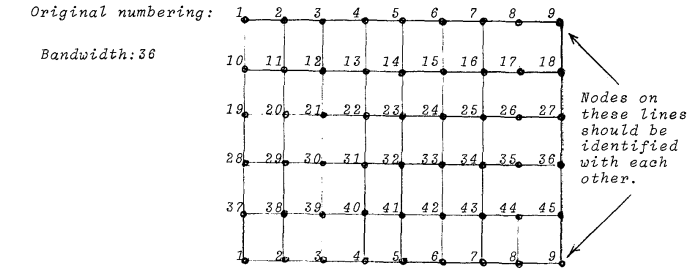
\includegraphics[width=0.49\linewidth]{figures/linear_cuthill-mckee_original.png}
    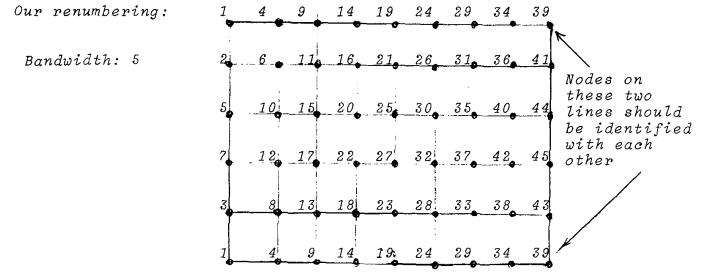
\includegraphics[width=0.49\linewidth]{figures/linear_cuthill-mckee_improved.png}
    \caption{Example from the original Cuthill--McKee paper~\cite{cuthill1969reducing}.}%
    \label{figure:linear_example_from_cuthill_mckee}
\end{figure}

\subsection{Exercices}%
\begin{exercise}
    [Inverse of Gaussian transformation]
    \label{exercise:inverse_gaussian_transformation}
    Prove the formula~\eqref{eq:inverse_gaussian_transformation}.
\end{exercise}

\begin{exercise}
    \label{exercise:linear_product_of_lower_triangular}
    Prove that the product of two lower triangular matrices is lower triangular.
\end{exercise}

\begin{exercise}
    \label{exercise:linear_positive_definite_matrix_nonsingular_principal_components}
    Assume that $\mat A \in \real^{n \times n}$ is positive definite,
    i.e.\ that
    \[
        \forall \vect x \in \real^n \backslash \{ \vect 0_n \}, \qquad \vect x^\t \mat A \vect x > 0.
    \]
    Show that all the principal submatrices of $\mat A$ are nonsingular.
\end{exercise}

\begin{compexercise}
    Implement the backward substitution algorithm for solving $\mat U x = y$.
    What is the computational cost of the algorithm?
\end{compexercise}

\begin{compexercise}
    \label{exercise:linear_lu_with_partial_pivoting}
    Compare the condition number of the matrices $\mat L$ and $\mat U$ with and without partial pivoting.
    For testing, use a matrix with pseudo-random entries generated as follows
    \begin{minted}{julia}
    import Random
    # Set the seed so that the code is deterministic
    Random.seed!(0)
    n = 1000 # You can change this parameter
    A = randn(n, n)
    \end{minted}
\end{compexercise}
\begin{solution}
    See the Jupyter notebook for this chapter.
\end{solution}

\begin{compexercise}
    \label{exercise:linear_cholesky}
    Write a code for calculating the Cholesky factorization of a symmetric positive definite matrix $\mat A$ by comparing the entries of the product $\mat C \mat C^\t$ with those of the matrix $\mat A$.
    What is the associated computational cost,
    and how does it compare with that of the $\mat L \mat U$ factorization?

    \noindent \textbf{Extra credit:} ... if your code is able to exploit the potential banded structure of the matrix passed as argument for better efficiency.
    Specifically, your code will be tested with a matrix is of the type \julia{BandedMatrix} defined in the \texttt{BandedMatrices.jl} package,
    which you will need to install.
    The following code can be useful for testing purposes.
    \begin{minted}{julia}
    import BandedMatrices
    import LinearAlgebra

    function cholesky(A)
        m, n = size(A)
        m != n && error("Matrix must be square")
        # Convert to banded matrix
        B = BandedMatrices.BandedMatrix(A)
        B.u != B.l && error("Matrix must be symmetric")
        # --> Your code comes here <--
    end
    n, u, l = 20000, 2, 2
    A = BandedMatrices.brand(n, u, l)
    A = A*A'
    # so that A is symmetric and positive definite (with probability 1).
    C = @time cholesky(A)
    LinearAlgebra.norm(C*C' - A, Inf)
    \end{minted}
    For information, my code takes about 1 second to run with the parameters given here.
\end{compexercise}

\begin{exercise}
    [Matrix square root]
    \label{exercise:matrix_square_root}
    Let $\mat A$ be a symmetric positive definite matrix.
    Show that $\mat A$ has a square root, i.e.\ that there exists a symmetric matrix $\mat B$ such that $\mat B \mat B = \mat A$.
\end{exercise}

\section{Iterative methods for linear systems}%
\label{sec:iterative_methods}
Iterative methods enjoy more flexibility than direct methods,
because they can be stopped at any point if the residue is deemed sufficiently small.
This generally enables to obtain a good solution at a computational cost that is significantly lower than that of direct methods.
In this section,
we present and study two classes of iterative methods:
basic iterative methods based on a splitting of the matrix $\mat A$,
and the so-called Krylov subspace methods.

\subsection{Basic iterative methods}%
\label{sub:basic_iterative_methods}
The basic iterative methods are particular cases of a general \emph{splitting method}.
Given a splitting of the matrix of the linear system as $\mat A = \mat M - \mat N$,
for a nonsingular matrix $\mat M \in \real^{n \times n}$ and a matrix $\mat N \in  \real^{n \times n}$,
together with an initial guess $\vect x^{(0)}$ of the solution,
one step of this general method reads
\begin{equation}
    \label{eq:linear_system_iterative_method}
    \mat M \vect x^{(k+1)} = \mat N \vect x^{(k)} + \vect b.
\end{equation}
For any choice of splitting,
the exact solution $\vect x$ to the linear system is a fixed point of this iteration,
in the sense that if $\vect x^{(0)} = \vect x$, then $\vect x^{(k)} = \vect x$ for all $k \geq 0$.
\Cref{eq:linear_system_iterative_method} is a linear system with matrix~$\mat M$,
unknown $\vect x^{(k+1)}$, and right-hand side $\mat N \vect x^{(k)} + \vect b$.
There is a compromise between the cost of a single step and the speed of convergence of the method.
In the extreme case where $\mat M = \mat A$ and $\mat N = 0$,
the method converges to the exact solution in one step,
but performing this step amounts to solving the initial problem.
In practice, in order for the method to be useful,
the linear system~\eqref{eq:linear_system_iterative_method} should be relatively simple to solve.
Concretely, this means that the matrix~$\mat M$ should be diagonal, triangular, block diagonal, or block triangular.
The error $\vect e^{(k)}$ and residue $\vect r^{(k)}$ at iteration $k$ are defined as follows:
\[
    \vect e^{(k)} = \vect x^{(k)} - \vect x,
    \qquad
    \vect r^{(k)} = \mat A \vect x^{(k)} - \vect b.
\]

\subsubsection{Convergence of the splitting method}%
\label{ssub:convergence_of_the_basic_splitting_method}
Before presenting concrete examples of splitting methods,
we obtain a necessary and sufficient condition for the convergence of~\eqref{eq:linear_system_iterative_method}
for any initial guess~$\vect x^{(0)}$.

\begin{proposition}
    [Convergence]
    \label{proposition:linear_convergence}
    The splitting method~\eqref{eq:linear_system_iterative_method} converges for any initial guess~$\vect x^{(0)}$
    if and only if $\rho(\mat M^{-1} \mat N) < 1$.
    In addition, for any $\varepsilon > 0$ there exists $K > 0$ such that
    \[
        \forall k \geq K,
        \qquad
        \norm{\vect e^{(k)}} \leq \bigl(\rho(A) + \varepsilon\bigr)^k \norm{\vect e^{(0)}}.
    \]
\end{proposition}
\begin{proof}
    Let us denote by $\vect x$ the solution to the linear system.
    Since $\mat M \vect x - \mat N \vect x = \vect b$,
    we have
    \[
        \mat M (\vect x^{(k+1)} - \vect x) = \mat N (\vect x^{(k)} - \vect x).
    \]
    Using the assumption that $\mat M$ is nonsingular,
    we obtain that the error satisfies the equation
    \[
        \vect e^{(k+1)} = (\mat M^{-1} \mat N) \vect e^{(k)}.
    \]
    Applying this equality repeatedly, we deduce
    \[
        \vect e^{(k+1)} = (\mat M^{-1} \mat N)^2 \vect e^{(k-1)} = \dots = (\mat M^{-1} \mat N)^{k+1} \vect e^{(0)}.
    \]
    Therefore,
    it holds that
    \[
        \forall k \geq 0, \qquad
        \norm{\vect e^{(k)}}
        \leq \norm[bigl]{(\mat M^{-1} \mat N)^{k}} \norm{\vect e^{(0)}}.
    \]
    In order to conclude the proof,
    we will used Gelfand's formula,
    proved in~\cref{proposition:matrices_gelfands} of \cref{cha:vectors_and_matrices}.
    This states that
    \[
        \lim_{k \to \infty} \norm[bigl]{(\mat M^{-1} \mat N)^{k}}^{\frac{1}{k}} = \rho(\mat M^{-1} \mat N).
    \]
    In particular, for all $\varepsilon > 0$ there is $K \in \nat$ such that
    \[
        \forall k \geq K, \qquad
        \norm[bigl]{(\mat M^{-1} \mat N)^{k}}^{\frac{1}{k}} \leq \rho(\mat M^{-1} \mat N) + \varepsilon.
    \]
    Rearranging this inequality gives that $\norm[bigl]{(\mat M^{-1} \mat N)^{k}} $ the statement.
\end{proof}

At this point,
it is natural to wonder whether there exist sufficient conditions on the matrix~$\mat A$ such that the inequality $\rho(\mat M^{-1} \mat N) < 1$ is satisfied,
which is best achieved on a case by case basis.
In the next sections,
we present four instances of splitting methods.
For each of them,
we obtain a sufficient condition for convergence.
We are particularly interested in the case where the matrix~$\mat A$ is symmetric (or Hermitian) and positive definite,
which often arises in applications,
and in the case where $\mat A$ is strictly row or column diagonally dominant.
We recall that a matrix $\mat A$ is said to be row or column diagonally dominant
if, respectively,
\[
    \lvert a_{ii} \rvert \geq \sum_{j \neq i} \lvert a_{ij} \rvert \quad \forall i
    \qquad \text{ or } \qquad
    \lvert a_{jj} \rvert \geq \sum_{i \neq j} \lvert a_{ij} \rvert \quad \forall j.
\]

\subsubsection{Richardson's method}%
\label{ssub:richardson_s_method}

Arguably the simplest splitting of the matrix $\mat A$ is given by $\mat A = \frac{1}{\omega} \mat I - \bigl(\frac{1}{\omega} \mat I - \mat A\bigr)$,
which leads to \emph{Richardson's method}:
\begin{equation}
    \label{eq:linear_richardson}
    \vect x^{(k+1)} = \vect x^{(k)} +  \omega (\vect b - \mat A \vect x^{(k)}).
\end{equation}
In this case the spectral radius which enters in the asymptotic rate of convergence is given by
\[
    \rho(\mat M^{-1} \mat N)
    = \rho\left(\omega \left(\frac{1}{\omega} \mat I - \mat A\right) \right)
    = \rho\bigl( \mat I - \omega \mat A \bigr)
\]
The eigenvalues of the matrix $\mat I - \omega \mat A$ are given by $1 - \omega \lambda_i$,
where $(\lambda_i)_{1 \leq i \leq L}$ are the eigenvalues of~$\mat A$.
Therefore, the spectral radius is given by
\[
    \rho(\mat M^{-1} \mat N)
    = \max_{1 \leq i \leq L} \abs{1  - \omega \lambda_i}.
\]

\paragraph{Case of symmetric positive definite $\mat A$.}%
\label{par:case_of_symmetric_positive_definite_mat_a_}
If the matrix $\mat A$ is symmetric and positive definite,
it is possible to explicitly calculate the optimal value of $\omega$ for convergence.
In order make convergence as fast as possible,
we want the spectral radius of $\mat M^{-1} \mat N$ to be as small as possible,
in view of~\cref{proposition:linear_convergence}.
Denoting by $\lambda_{\min}$ and $\lambda_{\max}$ the minimum and maximum eigenvalues of $\mat A$,
it is not difficult to show that
\[
    \rho(\mat M^{-1} \mat N)
    = \max_{1 \leq i \leq L} \abs{1  - \omega \lambda_i}
    = \max \bigl\{ \abs{1 - \omega \lambda_{\min}}, \abs{1 - \omega \lambda_{\max}}\bigr\}.
\]
The maximum is minimized when its two arguments are equal,
i.e.\ when $1 - \omega \lambda_{\min} = \omega \lambda_{\max} -1$.
From this we deduce the optimal value of $\omega$ and the associated spectral radius:
\[
    \omega_{\rm opt} = \frac{2}{\lambda_{\max} + \lambda_{\min}},
    \qquad
    \rho_{\rm opt}
    = 1 - \frac{2\lambda_{\min}}{\lambda_{\max} + \lambda_{\min}}
    = \frac{\lambda_{\max} - \lambda_{\min}}{\lambda_{\max} + \lambda_{\min}}
    =  \frac{\kappa_2(\mat A) - 1}{\kappa_2(\mat A) + 1}.
\]
We observe that the smaller the condition number of the matrix $\mat A$,
the better the asymptotic rate of convergence.

\begin{remark}
    [Link to optimization]
    In the case where $\mat A$ is symmetric and positive definite,
    the Richardson update~\eqref{eq:linear_richardson} may be viewed as a step of the steepest descent algorithm
    for the function $f(\vect x) = \frac{1}{2} \vect x^\t \mat A \vect x - \vect b^\t \vect x$:
    \begin{equation}
        \label{eq:linear_richardson_gradient}
        \vect x^{(k+1)} = \vect x^{(k)} - \omega \nabla f(\vect x^{(k)}).
    \end{equation}
    The gradient of this function is $\nabla f(\vect x) = \mat A \vect x - \vect b$,
    and its Hessian matrix is $\mat A$.
    Since the Hessian matrix is positive definite, the function is convex
    and attains its global minimum when $\nabla f$ is zero,
    i.e.\ when $\mat A x = \vect b$.
\end{remark}

\subsubsection{Jacobi's method}%
\label{ssub:jacobi_s_method}
In Jacobi's method, the matrix $\mat M$ in the splitting is the diagonal matrix $\mat D$ with the same entries as those of $\mat A$ on the diagonal.
We denote by $\mat L$ and $\mat U$ the lower and upper triangular parts of $\mat A$,
without the diagonal.
One step of the method reads
\begin{equation}
    \label{eq:linear_jacobi}
    \mat D \vect x^{(k+1)}
    = (\mat D - \mat A) \vect x^{(k)} + \vect b
    = - (\mat L + \mat U) \vect x^{(k)} + \vect b
\end{equation}
Since the matrix $\mat D$ on the left-hand side is diagonal,
this linear system with unknown $\vect x^{(k+1)}$ is very simple to solve.
The equation~\eqref{eq:linear_jacobi} can be rewritten equivalently as
\begin{equation*}
    \left\{
       \begin{aligned}
        & a_{11} x^{(\textcolor{darkblue}{k+1})}_1 + a_{12} x^{(k)}_2 + \dotsb + a_{1n} x^{(k)}_n = b_1 \\
        & a_{21} x^{(k)}_1 + a_{22} x^{(\textcolor{darkblue}{k+1})}_2 + \dotsb + a_{2n} x^{(k)}_n = b_2 \\
        & \vdots \\
        & a_{n1} x^{(k)}_1 + a_{n2} x^{(k)}_2 + \dotsb + a_{nn} x^{(\textcolor{darkblue}{k+1})}_n = b_n.
       \end{aligned}
   \right .
\end{equation*}
The updates for each of the entries of $\vect x^{(k+1)}$ are independent,
and so the Jacobi method lends itself well to parallel implementation.
The computational cost of one iteration,
measured in number of floating point operations required,
scales as $\mathcal O(n^2)$ if~$\mat A$ is a full matrix,
or $\mathcal O(nk)$ if~$\mat A$ is a sparse matrix with $k$ nonzero elements per row on average.
It is simple to prove the convergence of Jacobi's method is the case where $\mat A$ is diagonally dominant.
\begin{proposition}
    \label{proposition:linear_convergence_jacobi}
    Assume that $\mat A$ is strictly (row or column) diagonally dominant.
    Then it holds that $\rho(\mat M^{-1} \mat N) < 1$ for the Jacobi splitting.
\end{proposition}
\begin{proof}
    Assume that $\lambda$ is an eigenvalue of $\mat M^{-1} \mat N$
    and $\vect v$ is the associated unit eigenvector.
    Then
    \[
        \mat M^{-1} \mat N \vect v = \lambda \vect v
        \quad \Leftrightarrow \quad
        \mat N \vect v = \lambda \mat M \vect v
        \quad \Leftrightarrow \quad
        (\mat N - \lambda \mat M) \vect v = 0.
    \]
    In the case of Jacobi's splitting,
    this is equivalent to
    \[
        - (\mat L + \lambda \mat D + \mat U) \vect v = 0.
    \]
    If $\abs{\lambda} > 1$,
    then the matrix on the left-hand side of this equation is diagonally dominant and thus invertible
    (see \cref{exercise:invertibility_diagonal_dominant}).
    Therefore $\vect v = 0$, but this is a contradiction because $\vect v$ is vector of of unit norm.
    Consequently, all the eigenvalues are bounded from above strictly by 1 in modulus.
\end{proof}


\subsubsection{Gauss--Seidel's method}%
\label{ssub:gauss_seidel_s_method}

In Gauss Seidel's method, the matrix $\mat M$ in the splitting is the lower triangular part of $\mat A$,
including the diagonal.
One step of the method then reads
\begin{equation}
    \label{eq:linear_gauss_seidel}
    (\mat L + \mat D) \vect x^{(k+1)} = - \mat U \vect x^{(k)} + \vect b
\end{equation}
The system can be solved by forward substitution.
The equation~\eqref{eq:linear_gauss_seidel} can be rewritten equivalently as
\begin{equation*}
    \left\{
       \begin{aligned}
        & a_{11} x^{(\textcolor{darkblue}{k+1})}_1 + a_{12} x^{(k)}_2 + a_{13} x^{(k)}_3 + \dotsb + a_{1n} x^{(k)}_n = b_1 \\
        & a_{21} x^{(\textcolor{darkblue}{k+1})}_1 + a_{22} x^{(\textcolor{darkblue}{k+1})}_2 + a_{23} x^{(k)}_3 + \dotsb + a_{2n} x^{(k)}_n = b_2 \\
        & a_{32} x^{(\textcolor{darkblue}{k+1})}_1 + a_{32} x^{(\textcolor{darkblue}{k+1})}_2 + a_{33} x^{(\textcolor{darkblue}{k+1})}_3 + \dotsb + a_{3n} x^{(k)}_n = b_2 \\
        & \vdots \\
        & a_{n1} x^{(\textcolor{darkblue}{k+1})}_1 + a_{n2} x^{(\textcolor{darkblue}{k+1})}_2 + a_{n3} x^{(\textcolor{darkblue}{k+1})}_3 + \dotsb + a_{nn} x^{(\textcolor{darkblue}{k+1})}_n = b_n.
       \end{aligned}
   \right .
\end{equation*}
Given $\vect x^{(k)}$,
the first entry of $\vect x^{(k+1)}$ can be obtained from the first equation.
Then the value of the second entry can be obtained from the second equation, etc.
Unlike Jacobi's method,
the Gauss--Seidel method is sequential and the entries of $\vect x^{(k+1)}$ cannot be updated in parallel.

It is possible to prove the convergence of the Gauss--Seidel method in particular cases.
For example, the method converges if $\mat A$ is strictly diagonally dominant.
Proving this,
using an approach similar to that in the proof of~\cref{proposition:linear_convergence_jacobi},
is the goal of~\cref{exercise:linear_convergence_gauss_seidel}.
It is also possible to prove convergence when $\mat A$ is Hermitian and positive definite.
We show this in the next section for the relaxation method,
which generalizes the Gauss--Seidel method.

\subsubsection{Relaxation method}%

The relaxation method generalizes the Gauss--Seidel method.
It corresponds to the splitting
\begin{equation}
    \mat A = \left( \frac{\mat D}{\omega} + \mat L \right) - \left(\frac{1 - \omega}{\omega} \mat D - \mat U \right).
\end{equation}
When $\omega = 1$,
this is simply the Gauss--Seidel splitting.
The idea is that,
by letting $\omega$ be a parameter that can differ from 1,
faster convergence can be achieved.
This intuition will be verified later.
The equation~\eqref{eq:linear_system_iterative_method} for this splitting can be rewritten equivalently as
\begin{equation*}
    \left\{
       \begin{aligned}
        & a_{11} \bigl(x^{(\textcolor{darkblue}{k+1})}_1 - x^{(k)}_1 \bigr) =  \omega \left(a_{11} x^{(k)}_1 + a_{12} x^{(k)}_2 + \dotsb + a_{1n} x^{(k)}_n - b_1 \right) \\
        & a_{22} \bigl(x^{(\textcolor{darkblue}{k+1})}_2 - x^{(k)}_2 \bigr) =  \omega \left(a_{21} x^{(\textcolor{darkblue}{k+1})}_1 + a_{22} x^{(k)}_2 + \dotsb + a_{2n} x^{(k)}_n - b_2 \right) \\
        & \vdots \\
        & a_{nn} \bigl(x^{(\textcolor{darkblue}{k+1})}_n - x^{(k)}_n \bigr) =  \omega \left(a_{n1} x^{(\textcolor{darkblue}{k+1})}_1 + a_{n2} x^{(\textcolor{darkblue}{k+1})}_2 + \dotsb + a_{nn} x^{(k)}_n - b_n \right).
       \end{aligned}
   \right .
\end{equation*}
The coefficient on the right-hand side is larger than in the Gauss--Seidel method if $\omega > 1$,
and smaller if $\omega < 1$.
These regimes are called \emph{over-relaxation} and \emph{under-relaxation}, respectively.

To conclude this section,
we establish a sufficient condition for the convergence of the relaxation method,
and also of the Gauss--Seidel method as a particular case when $\omega = 1$,
when the matrix $\mat A$ is Hermitian and positive definite.
To this end, we begin by showing the following preparatory result,
which concerns a general splitting $\mat A = \mat M - \mat N$.
\begin{proposition}
    \label{proposition:criterion_convergence}
    Let $\mat A$ be Hermitian and positive definite.
    If the Hermitian matrix $\mat M^* + \mat N$ is positive definite,
    then $\rho(\mat M^{-1} \mat N) < 1$.
\end{proposition}
\begin{proof}
    First, notice that $\mat M + \mat N^*$ is indeed Hermitian because
    \[
        (\mat M + \mat N^*)^* = \mat M^* + \mat N = \mat A^* + \mat N^* + \mat N = \mat A + \mat N^* + \mat N.
    \]
    We will show that $\norm{\mat M^{-1} \mat N}_{\mat A} < 1$,
    where $\norm{\placeholder}_{\mat A}$ is the matrix norm induced by the following norm on vectors:
    \[
        \norm{\vect x}_{\mat A} := \sqrt{\vect x^* \mat A \vect x}.
    \]
    Showing that this indeed defines a vector norm is the goal of~\cref{exercise:linear_norm_induced_A}.
    Since $\mat N = \mat M - \mat A$, it holds that
    \(
        \norm{\mat M^{-1} \mat N}_{\mat A}
        = \norm{\mat I - \mat M^{-1} \mat A}_{\mat A},
    \)
    and so
    \[
        \norm{\mat M^{-1} \mat N}_{\mat A}
        = \sup \bigl\{ \norm{\vect x - \mat M^{-1} \mat A \vect x}_{\mat A}: \norm{\vect x}_{\mat A} \leq 1 \bigr\}.
    \]
    Letting $\vect y = \mat M^{-1} \mat A \vect x$, we calculate
    \begin{align*}
        \forall \vect x \in \real^n \text{~with~} \norm{\vect x}_{\mat A} \leq 1, \quad
        \norm{\vect x - \mat M^{-1} \mat A \vect x}_{\mat A}^2
        &= \vect x^* \mat A \vect x - \vect y^* \mat A \vect x - \vect x^* \mat A \vect y + \vect y^* \mat A \vect y \\
        &= \vect x^* \mat A \vect x - \vect y^* \mat M \mat M^{-1} \mat A \vect x - (\mat M^{-1} \mat A \vect x)^* \mat M^* \vect y + \vect y^* \mat A \vect y \\
        &= \vect x^* \mat A \vect x - \vect y^* \mat M \vect y - \vect y^* \mat M^* \vect y + \vect y^* (\mat M - \mat N) \vect y \\
        &= \vect x^* \mat A \vect x - \vect y^* (\mat M^* + \mat N) \vect y \leq 1 - \vect y^* (\mat M^* + \mat N) \vect y < 1,
        % &= \vect x^\t \mat A \vect x - 2 \vect y^\t \mat M \vect \vect y + \vect y^\t \mat A \vect y \\
    \end{align*}
    where we used in the last inequality the assumption that $\mat M^* + \mat N$ is positive definite.
    This shows that \( \norm{\mat M^{-1} \mat N}_{\mat  A} < 1\), and so $\rho(\mat M^{-1} \mat N) < 1$.
\end{proof}

As a corollary,
we obtain a sufficient condition for the convergence of the relaxation method.
\begin{corollary}
    \label{corollary:convergence_relaxation}
    Assume that $\mat A$ is Hermitian and positive definite.
    Then the relaxation method converges if $\omega \in (0, 2)$.
\end{corollary}
\begin{proof}
    For the relaxation method,
    we have
    \[
        \mat M + \mat N^*
        = \left( \frac{\mat D}{\omega} + \mat L \right) + \left(\frac{1 - \omega}{\omega} \mat D - \mat U \right)^*.
    \]
    Since $\mat A$ is Hermitian,
    it holds that $\mat D^* = \mat D$ and $\mat U^* = \mat L$.
    Therefore,
    \[
        \mat M + \mat N^*
        = \frac{2 - \omega}{\omega} \mat D.
    \]
    The diagonal elements of $\mat D$ are all positive,
    because $\mat A$ is positive definite.
    (Indeed, if there was an index $i$ such that $d_{ii} \leq 0$,
    then it would hold that $\vect e_i^\t \mat A \vect e_i = d_{ii} \leq 0$,
    contradicting the assumption that $\mat A$ is positive definite.)
    We deduce that $\mat M + \mat N^*$ is positive definite if and only if $\omega \in (0, 2)$.
    We can then conclude the proof by using \cref{proposition:criterion_convergence}.
\end{proof}
Note that \cref{corollary:convergence_relaxation} implies as a particular case
the convergence of the Gauss--Seidel method when $\mat A$ is Hermitian and positive definite.
The condition $\omega \in (0, 2)$ is fact necessary for the convergence of the relaxation method,
not only in the case of a Hermitian positive definite matrix $\mat A$ but in general.
\begin{proposition}
    Let $\mat A \in \complex^{n \times n}$ be an invertible matrix,
    and let $\mat A = \mat M_{\omega} - \mat N_{\omega}$ denote the splitting of the relaxation method with parameter~$\omega$.
    It holds that
    \[
        \forall \omega \neq 0, \qquad
        \rho(\mat M_{\omega}^{-1} \mat N_{\omega})
        \geq \abs{\omega - 1}.
    \]
\end{proposition}
\begin{proof}
    We recall the following facts:
    \begin{itemize}
        \item the determinant of a product of matrices is equal to the product of the determinants.
        \item the determinant of a triangular matrix is equal to the product of its diagonal entries;
        \item the determinant of a matrix is equal to the product of its eigenvalues,
            to the power of their algebraic multiplicity.
            This can be shown for the previous two item,
            by passing to the Jordan normal form.
    \end{itemize}
    Therefore,
    we have that
    \[
        \det (\mat M_{\omega}^{-1} \mat N_{\omega}) = \det (\mat M_{\omega})^{-1}  \det (\mat N_{\omega})
        = \frac {\det \left(\frac{1 - \omega}{\omega} \mat D - \mat U \right)}{\det \left( \frac{\mat D}{\omega} + \mat L \right)}
        = (1 - \omega)^n.
    \]
    Since the determinant on the left-hand side is the product of the eigenvalues of $\mat M_{\omega}^{-1} \mat N_{\omega}$,
    it is bounded from above in modulus by $\rho(\mat M_{\omega}^{-1} \mat N_{\omega})^n$,
    and so we deduce $\rho(\mat M_{\omega}^{-1} \mat N_{\omega})^n \geq \abs{1 - \omega}^n$.
    The statement then follows by taking the $n$-th root.
\end{proof}

\subsubsection{Monitoring the convergence}
\label{ssub:monitoring_the_convergence}
In practice,
we have access to the residue $\vect r^{(k)} = \mat A \vect x^{(k)} - \vect b$ at each iteration,
but not to the error $\vect e^{(k)} = \vect x^{(k)} - \vect x$,
as calculating the latter would require to know the exact solution of the problem.
Nevertheless,
the two are related by the equation
\[
    \vect r^{(k)} = \mat A \vect e^{(k)}
    \quad \Leftrightarrow \quad \vect e^{(k)} = \mat A^{-1} \vect r^{(k)}.
\]
Therefore, it holds that $\norm{\vect e^{(k)}} \leq \norm{\mat A^{-1}} \norm{\vect r^{(k)}}$.
Likewise, the relative error satisfies
\[
     \frac{\norm{\vect e^{(k)}}}{\norm{\vect x}}
     = \frac{\norm{\mat A^{-1} \vect r^{(k)}}}{\norm{\mat A^{-1} \vect b}}
\]
and since $\norm{\vect b} = \norm{\mat A \mat A^{-1} \vect b} \leq \norm{\mat A} \norm{\mat A^{-1} \vect b}$,
we deduce
\[
     \frac{\norm{\vect e^{(k)}}}{\vect x}
     \leq \kappa(\mat A) \frac{\norm{\vect r^{(k)}}}{\norm{\vect b}}.
\]
The fraction on the right-hand side is the \emph{relative residue}.
If the system is well conditioned,
that is if $\kappa(A)$ is close to one,
then controlling the residue enables a good control of the error.

\subsubsection{Stopping criterion}%
\label{ssub:stopping_criterion}

In practice,
several criteria can be employed to determine when to stop iterating.
Given a small number $\varepsilon$ (unrelated to the machine epsilon in \cref{cha:rounding_errors}),
the following alternatives are available:
\begin{itemize}
    \item
        Stop when $\vect r^{(k)} \leq \varepsilon$.
        The downside of this approach is that
        it is not \emph{scaling invariant}:
        when used for solving the following rescaled system
        \[
            k \mat A \vect x = k \vect b, \qquad k \neq 1,
        \]
        a splitting method with rescaled initial guess $k \vect x^{(0)}$
        will require a number of iterations that depends on $k$:
        fewer if $k \ll 1$ and more if $k \gg 1$.
        In practice, controlling the relative residue and the relative error is often preferable.

    \item
        Stop when $\norm{\vect r^{(k)}} / \norm{\vect r^{(0)}} \leq \varepsilon$.
        This criterion is scaling invariant,
        but the number of iterations is dependent on the quality of the initial guess $\vect x^{(0)}$.

    \item
        Stop when $\norm{\vect r^{(k)}} / \norm{\vect b}$.
        This criterion is generally the best,
        because it is both scaling invariant and the quality of the final iterate is independent of that of the initial guess.
\end{itemize}

\subsection{Exercises}%

\begin{exercise}
    \label{exercise:invertibility_diagonal_dominant}
    Show that if $\mat A$ is row or column diagonally dominant,
    then $\mat A$ is invertible.
\end{exercise}

\begin{exercise}
    Let $\mat T$ be a nonsingular matrix.
    Show that
    \[
        \norm{\mat A}_{\mat T} := \norm{\mat T^{-1} \mat A \mat T}_2
    \]
    defines a matrix norm induced by a vector norm.
\end{exercise}

\begin{exercise}
    \label{exercise:linear_norm_induced_A}
    Let $\mat A \in \real^{n \times n}$ be a symmetric positive definite matrix.
    Show that the functional
    \[
        \norm{\placeholder}_{\mat A}: \vect x \mapsto \sqrt{\vect x^\t \mat A \vect x}
    \]
    defines a norm on $\real^n$.
\end{exercise}

\begin{exercise}
    Show that the residue satisfies the equation
    \[
        \vect r^{(k+1)} = \mat N \mat M^{-1} \vect r^{(k)} = (\mat I - \mat A \mat M^{-1}) \vect r^{(k)}.
    \]
\end{exercise}

\begin{exercise}
    Show that, if $\mat A$ and $\mat B$ are two square matrices,
    then $\rho(\mat A \mat B) = \rho(\mat B \mat A)$.
\end{exercise}

\begin{exercise}
    Is $\rho(\placeholder)$ a norm? Prove or disprove.
\end{exercise}

\begin{exercise}
    Prove that, if $\mat A$ is a diagonal matrix, then
    \[
        \norm{\mat A}_1 = \norm{\mat A}_2 = \norm{\mat A}_{\infty} = \rho(\mat A).
    \]
\end{exercise}

\begin{exercise}
    Show that, for any matrix norm $\norm{\placeholder}$ induced by a vector norm,
    \[
        \rho(\mat A) \leq \norm{\mat A}.
    \]
\end{exercise}

\begin{exercise}
    Let $\norm{\placeholder}$ denote the Euclidean vector norm on $\real^n$.
    We define in~\cref{cha:vectors_and_matrices} the induced matrix norm as
    \[
        \norm{\mat A} = \sup \bigl\{ \norm{\mat A \vect x}: \norm{\vect x} \leq 1 \bigr\}.
    \]
    Show from this definition that, if $\mat A$ is symmetric and positive definite,
    then
    \[
        \norm{\mat A} = \norm{\mat A}_* := \sup \bigl\{ \abs{\vect x^\t \mat A \vect x}: \norm{\vect x} \leq 1 \bigr\}.
    \]
    % What is the induced matrix norm on $\real^{n \times n}$?
\end{exercise}
\begin{solution}
    By the Cauchy--Schwarz inequality and the definition of $\norm{\mat A}$,
    it holds that
    \[
        \forall \vect x \in \real^n \text{ with } \norm{\vect x} \leq 1, \qquad
         \abs{\vect x^\t \mat A \vect x}
         \leq \norm{\vect x} \norm{\mat A \vect x}
         \leq \norm{\vect x} \norm{\mat A} \norm{\vect x} \leq \norm{\mat A}.
    \]
    This shows that $\norm{\mat A}_* \leq \norm{\mat A}$.
    Conversely,
    letting $\mat B$ denote a matrix square root of $\mat A$ (see \cref{exercise:matrix_square_root}),
    we have
    \begin{align*}
        \forall \vect x \in \real^n \text{ with } \norm{\vect x} \leq 1, \qquad
        \norm{\mat A \vect x}
        &= \sqrt{\vect x^\t \mat A^\t \mat A \vect x}
        = \sqrt{(\mat B\vect x)^\t \mat B \mat B (\mat B\vect x)}
        = \sqrt{(\mat B\vect x)^\t \mat A (\mat B\vect x)} \\
        &= \norm{\mat B \vect x} \sqrt{\vect y^\t \mat A \vect y},
        \qquad \vect y = \frac{\mat B \vect x}{\norm{\mat B \vect x}}.
    \end{align*}
    It holds that $\norm{\mat B \vect x} = \sqrt{\vect x^\t \mat A \vect x} \leq \sqrt{\norm{\mat A}_*}$.
    In addition $\norm{\vect y} = 1$,
    so the expression inside the square root is bounded from above by $\norm{\mat A}_*$,
    which enables to conclude the proof.
\end{solution}

\begin{compexercise}
    Implement an iterative method based on a splitting for finding a solution to the following linear system on $\real^n$.
    \[
        \frac{1}{h^2}
        \begin{pmatrix}
            2 & -1 \\
            -1 & 2  & -1 \\
               & -1 & 2      & -1 \\
               &    & \ddots & \ddots & \ddots & \\
               &    &        & -1    & 2      & -1 \\
               &    &        &     & -1      & 2 \\
        \end{pmatrix}
        \begin{pmatrix}
            x_1 \\
            x_2 \\
            x_3 \\
            \vdots \\
            x_{n-1} \\
            x_n \\
        \end{pmatrix}
        =
        \begin{pmatrix}
            1 \\
            1 \\
            1 \\
            \vdots \\
            1 \\
            1
        \end{pmatrix},
        \qquad
        h = \frac{1}{n}.
    \]
    Plot the norm of the residue as a function of the iteration index.
    Use as stopping criterion the condition
    \[
        \norm{\vect r^{(k)}} \leq \varepsilon \norm{\vect b},
        \qquad \varepsilon = 10^{-10}.
    \]
    The code will be tested with $n = 20,\!000$.
\end{compexercise}

\begin{exercise}
    \label{exercise:linear_convergence_gauss_seidel}
    Prove that, if the matrix $\mat A$ is strictly diagonally dominant (by rows or columns),
    then the Gauss--Seidel method converges, i.e.\ $\rho(\mat M^{-1} \mat N) < 1$.
    You can use the same approach as in the proof of \cref{proposition:linear_convergence_jacobi}.
\end{exercise}


% \begin{minted}{julia}
% \end{minted}

\begin{center}

\begin{tikzpicture}[limb/.style={line cap=round,line width=1.5mm,line join=bevel}]
\draw[line width=2mm,rounded corners,fill=yellow] (-2,0) -- (0,-2) -- (2,0) -- (0,2) -- cycle;
\fill (1.5mm,7mm) circle (1.5mm);
\fill(0,-7.5mm) -- ++(10mm,0mm) -- ++(120:2mm)--++(100:1mm)--++(150:2mm) arc (70:170:2.5mm and 1mm);
\draw[limb] (-7.5mm,-6.5mm)--++(70:4mm)--++(85:4mm) coordinate(a)--++(-45:5mm)--(-2.5mm,-6.5mm);
\fill[rotate around={45:(a)}] ([shift={(-0.5mm,0.55mm)}]a) --++(0mm,-3mm)--++
        (7mm,-0.5mm)coordinate(b)--++(0mm,4mm)coordinate(c)--cycle;
\draw[limb] ([shift={(-0.6mm,-0.4mm)}]b) --++(-120:5mm) ([shift={(-0.5mm,-0.5mm)}]c) --++
        (-3mm,0mm)--++(-100:3mm)coordinate (d);
\draw[ultra thick] (d) -- ++(-45:1.25cm);
\end{tikzpicture}
\textcolor{red}{Work in progress}
\end{center}
